% Created by tikzDevice version 0.12.6 on 2026-11-16 07:45:26
% !TEX encoding = UTF-8 Unicode
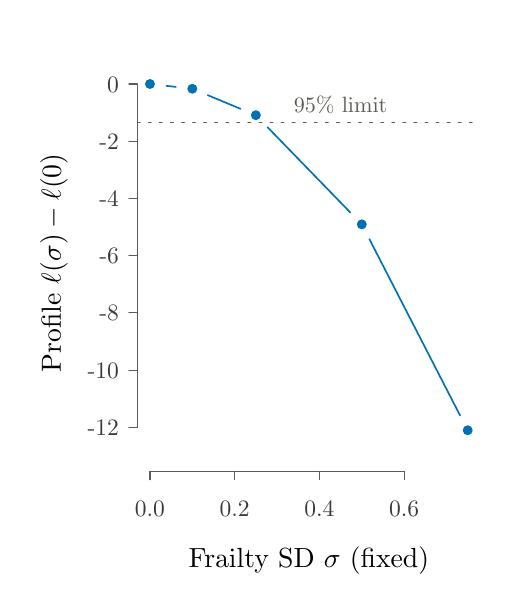
\begin{tikzpicture}[x=1pt,y=1pt]
\definecolor{fillColor}{RGB}{255,255,255}
\path[use as bounding box,fill=fillColor,fill opacity=0.00] (0,0) rectangle (168.39,198.74);
\begin{scope}
\path[clip] ( 39.60, 38.40) rectangle (163.59,189.14);
\definecolor{drawColor}{RGB}{0,114,178}

\path[draw=drawColor,line width= 0.6pt,line join=round,line cap=round] ( 50.15,177.72) -- ( 53.54,177.34);

\path[draw=drawColor,line width= 0.6pt,line join=round,line cap=round] ( 65.04,174.36) -- ( 76.92,169.41);

\path[draw=drawColor,line width= 0.6pt,line join=round,line cap=round] ( 86.64,162.80) -- (116.55,131.98);

\path[draw=drawColor,line width= 0.6pt,line join=round,line cap=round] (123.47,122.34) -- (156.25, 58.60);
\definecolor{fillColor}{RGB}{0,114,178}

\path[fill=fillColor] ( 44.19,178.39) circle (  1.80);

\path[fill=fillColor] ( 59.50,176.67) circle (  1.80);

\path[fill=fillColor] ( 82.46,167.11) circle (  1.80);

\path[fill=fillColor] (120.73,127.67) circle (  1.80);

\path[fill=fillColor] (159.00, 53.27) circle (  1.80);
\end{scope}
\begin{scope}
\path[clip] (  0.00,  0.00) rectangle (168.39,198.74);
\definecolor{drawColor}{RGB}{92,91,85}

\path[draw=drawColor,line width= 0.4pt,line join=round,line cap=round] ( 44.19, 38.40) -- (136.04, 38.40);

\path[draw=drawColor,line width= 0.4pt,line join=round,line cap=round] ( 44.19, 38.40) -- ( 44.19, 35.40);

\path[draw=drawColor,line width= 0.4pt,line join=round,line cap=round] ( 74.81, 38.40) -- ( 74.81, 35.40);

\path[draw=drawColor,line width= 0.4pt,line join=round,line cap=round] (105.42, 38.40) -- (105.42, 35.40);

\path[draw=drawColor,line width= 0.4pt,line join=round,line cap=round] (136.04, 38.40) -- (136.04, 35.40);
\definecolor{drawColor}{RGB}{59,58,53}

\node[text=drawColor,anchor=base,inner sep=0pt, outer sep=0pt, scale=  0.85] at ( 44.19, 22.20) {0.0};

\node[text=drawColor,anchor=base,inner sep=0pt, outer sep=0pt, scale=  0.85] at ( 74.81, 22.20) {0.2};

\node[text=drawColor,anchor=base,inner sep=0pt, outer sep=0pt, scale=  0.85] at (105.42, 22.20) {0.4};

\node[text=drawColor,anchor=base,inner sep=0pt, outer sep=0pt, scale=  0.85] at (136.04, 22.20) {0.6};
\definecolor{drawColor}{RGB}{92,91,85}

\path[draw=drawColor,line width= 0.4pt,line join=round,line cap=round] ( 39.60, 54.32) -- ( 39.60,178.39);

\path[draw=drawColor,line width= 0.4pt,line join=round,line cap=round] ( 39.60, 54.32) -- ( 36.60, 54.32);

\path[draw=drawColor,line width= 0.4pt,line join=round,line cap=round] ( 39.60, 75.00) -- ( 36.60, 75.00);

\path[draw=drawColor,line width= 0.4pt,line join=round,line cap=round] ( 39.60, 95.68) -- ( 36.60, 95.68);

\path[draw=drawColor,line width= 0.4pt,line join=round,line cap=round] ( 39.60,116.36) -- ( 36.60,116.36);

\path[draw=drawColor,line width= 0.4pt,line join=round,line cap=round] ( 39.60,137.03) -- ( 36.60,137.03);

\path[draw=drawColor,line width= 0.4pt,line join=round,line cap=round] ( 39.60,157.71) -- ( 36.60,157.71);

\path[draw=drawColor,line width= 0.4pt,line join=round,line cap=round] ( 39.60,178.39) -- ( 36.60,178.39);
\definecolor{drawColor}{RGB}{59,58,53}

\node[text=drawColor,anchor=base east,inner sep=0pt, outer sep=0pt, scale=  0.85] at ( 33.00, 51.39) {-12};

\node[text=drawColor,anchor=base east,inner sep=0pt, outer sep=0pt, scale=  0.85] at ( 33.00, 72.07) {-10};

\node[text=drawColor,anchor=base east,inner sep=0pt, outer sep=0pt, scale=  0.85] at ( 33.00, 92.75) {-8};

\node[text=drawColor,anchor=base east,inner sep=0pt, outer sep=0pt, scale=  0.85] at ( 33.00,113.43) {-6};

\node[text=drawColor,anchor=base east,inner sep=0pt, outer sep=0pt, scale=  0.85] at ( 33.00,134.11) {-4};

\node[text=drawColor,anchor=base east,inner sep=0pt, outer sep=0pt, scale=  0.85] at ( 33.00,154.78) {-2};

\node[text=drawColor,anchor=base east,inner sep=0pt, outer sep=0pt, scale=  0.85] at ( 33.00,175.46) {0};
\end{scope}
\begin{scope}
\path[clip] (  0.00,  0.00) rectangle (168.39,198.74);
\definecolor{drawColor}{RGB}{0,0,0}

\node[text=drawColor,anchor=base,inner sep=0pt, outer sep=0pt, scale=  1.00] at (101.59,  3.60) {Frailty SD $\sigma$ (fixed)};

\node[text=drawColor,rotate= 90.00,anchor=base,inner sep=0pt, outer sep=0pt, scale=  1.00] at ( 12.00,113.77) {Profile $\ell(\sigma) - \ell(0)$};
\end{scope}
\begin{scope}
\path[clip] ( 39.60, 38.40) rectangle (163.59,189.14);
\definecolor{drawColor}{RGB}{92,91,85}

\path[draw=drawColor,line width= 0.4pt,dash pattern=on 1pt off 3pt ,line join=round,line cap=round] ( 39.60,164.40) -- (163.59,164.40);

\node[text=drawColor,anchor=base,inner sep=0pt, outer sep=0pt, scale=  0.80] at (113.08,168.00) {95\% limit};
\end{scope}
\end{tikzpicture}
